% !TEX TS-program = xelatex
\documentclass[a4paper,10pt]{report}
% Thông tin dùng chung cho báo cáo và slide.
% Kiểm tra mã môn, lớp, học kỳ, năm học và giảng viên trước khi nộp.
\newcommand{\reporttitle}{BÁO CÁO ĐỒ ÁN: CLIPSeg}
\newcommand{\projecttopic}{Phân đoạn ảnh với text và visual prompt}
\newcommand{\groupname}{Cá nhân}
\newcommand{\coursename}{Ứng dụng xử lý ảnh và video số}
\newcommand{\courseschedule}{[Điền lịch học]}
\newcommand{\coursecode}{[Điền mã môn]}
\newcommand{\classname}{[Điền lớp]}
\newcommand{\semester}{[Điền học kỳ]}
\newcommand{\academicyear}{[Điền năm học]}
\newcommand{\studentone}{Lưu Huy Minh Quang}
\newcommand{\studentoneid}{23127016}
\newcommand{\studentoneemail}{lhmquang232@clc.fitus.edu.vn}
\newcommand{\studentonemajor}{Thị giác máy tính}
\newcommand{\advisorone}{[Điền giảng viên phụ trách]}
\newcommand{\reportplace}{Thành phố Hồ Chí Minh}
\newcommand{\reportdate}{tháng 10 năm 2026}

\usepackage[left=0.75in,right=0.75in,top=1in,bottom=1in]{geometry}
\usepackage{fontspec}
\usepackage{polyglossia}
\usepackage{setspace}
\usepackage{graphicx}
\usepackage[table]{xcolor}
\usepackage{tikz}
\usetikzlibrary{calc,arrows.meta,shapes.geometric}
\usepackage{float}
\usepackage{placeins}
\usepackage{amsmath}
\usepackage{amssymb}
\usepackage{enumitem}
\usepackage{xurl}
\usepackage{microtype}
\usepackage{longtable}
\usepackage{tabularx}
\usepackage{booktabs}
\usepackage{array}
\usepackage{textcomp}
\usepackage{algorithm}
\usepackage{algpseudocode}
\usepackage[hidelinks]{hyperref}
\usepackage[style=ieee,backend=biber,language=english]{biblatex}

\setmainfont{Latin Modern Roman}
\setsansfont{Latin Modern Sans}
\setmonofont{Latin Modern Mono}

\setmainlanguage{vietnamese}
\setotherlanguage{english}
\DeclareLanguageMapping{vietnamese}{english}

\graphicspath{{figures/}{assets/}}
\setstretch{1.15}
\setcounter{secnumdepth}{3}
\setcounter{tocdepth}{3}
\emergencystretch=2em
\hbadness=10000
\vbadness=10000

\addbibresource{references.bib}
\AtBeginBibliography{\sloppy}

\addto\captionsvietnamese{%
  \renewcommand{\contentsname}{Mục lục}%
  \renewcommand{\listfigurename}{Danh sách hình vẽ}%
  \renewcommand{\listtablename}{Danh sách bảng}%
  \renewcommand{\figurename}{Hình}%
  \renewcommand{\tablename}{Bảng}%
  \renewcommand{\chaptername}{Chương}%
}
\floatname{algorithm}{Thuật toán}
\algrenewcommand\algorithmicrequire{\textbf{Input:}}
\algrenewcommand\algorithmicensure{\textbf{Output:}}

\BeforeBeginEnvironment{itemize}{\par}
\setlist[itemize]{leftmargin=*,labelsep=0.5em}
\setlist[itemize,2]{label=\textopenbullet}

\newcolumntype{Y}{>{\centering\arraybackslash}X}
\newcolumntype{L}{>{\raggedright\arraybackslash}X}

\newcommand{\maybeincludegraphics}[2][0.92\textwidth]{%
  \IfFileExists{#2}{%
    \includegraphics[width=#1]{#2}%
  }{%
    \fbox{\parbox[c][0.22\textheight][c]{0.86\textwidth}{\centering Chèn hình\\\texttt{\detokenize{#2}}}}%
  }%
}

\newcommand{\labfigure}[4][0.92\textwidth]{%
  \begin{figure}[H]
    \centering
    \maybeincludegraphics[#1]{#2}
    \caption{#3}
    \label{#4}
  \end{figure}
}


\begin{document}
% ======================
% Title page
% ======================
\begin{titlepage}
  \thispagestyle{empty}

  \begin{tikzpicture}[overlay, remember picture]
    \draw [line width=3pt]
      ($ (current page.north west) + (2.0cm, -2.0cm) $)
      rectangle
      ($ (current page.south east) + (-2.0cm, 2.0cm) $);
    \draw [line width=0.5pt]
      ($ (current page.north west) + (2.1cm, -2.1cm) $)
      rectangle
      ($ (current page.south east) + (-2.1cm, 2.1cm) $);
    \draw [line width=0.5pt]
      ($ (current page.north west) + (1.9cm, -1.9cm) $)
      rectangle
      ($ (current page.south east) + (-1.9cm, 1.9cm) $);
  \end{tikzpicture}

  \begin{center}
    \textbf{\fontsize{14pt}{0pt}\selectfont TRƯỜNG ĐẠI HỌC KHOA HỌC TỰ NHIÊN, ĐHQG-HCM}\\
    \vspace{6pt}
    \textbf{\fontsize{14pt}{0pt}\selectfont KHOA CÔNG NGHỆ THÔNG TIN}\\
    \vspace{72pt}

    \IfFileExists{assets/HCMUS.png}{%
      
\includegraphics[width=0.48\textwidth]{assets/HCMUS.png}\\
    }{%
      \fbox{\parbox[c][0.18\textheight][c]{0.48\textwidth}{\centering\Large\bfseries LOGO}}\\
    }

    \vspace{0.8cm}
    \textbf{\fontsize{18pt}{22pt}\selectfont \reporttitle}\\[0.25cm]

    \vspace{0.8cm}
    {\fontsize{12pt}{0pt}\selectfont Hình thức: \groupname}\\[6pt]
    {\fontsize{12pt}{0pt}\selectfont Đề tài: \projecttopic}\\[6pt]
    {\fontsize{12pt}{0pt}\selectfont Môn học: \coursename}\\[6pt]
    {\fontsize{12pt}{0pt}\selectfont Lớp: \classname}\\

    \vspace{1cm}

    \begin{tabular}{l l}
      \textbf{Giảng viên:} & \advisorone \\[6pt]
      \textbf{Sinh viên:}  & \studentone{} -- \studentoneid \\[6pt]
    \end{tabular}

    \vfill
     {\reportplace, \reportdate}
  \end{center}
\end{titlepage}

\fontsize{10pt}{12.5pt}\selectfont
\chapter*{Lời nói đầu}
\addcontentsline{toc}{chapter}{Lời nói đầu}

Báo cáo tập trung vào mô hình CLIPSeg trong bài toán phân đoạn ảnh theo câu nhắc văn bản hoặc ảnh mẫu. Nội dung gồm khảo sát phương pháp, thiết kế đánh giá trên tập nhỏ và phân tích ảnh hưởng của prompt.

\medskip
\noindent\textbf{Nội dung cần hoàn thiện:} Viết lời giới thiệu theo quá trình thực hiện thực tế và bổ sung lời cảm ơn phù hợp trước khi nộp.

\vspace{1cm}
\begin{flushright}
\textit{Sinh viên thực hiện}\\
\textit{\studentone}
\end{flushright}

\chapter*{Thông tin chung}
\addcontentsline{toc}{chapter}{Thông tin chung}
\begin{tabular}{p{0.28\textwidth}p{0.66\textwidth}}
\textbf{Hình thức:} & \groupname \\[6pt]
\textbf{Đề tài:} & \projecttopic \\[6pt]
\textbf{Môn học:} & \coursename \\[6pt]
\textbf{Lịch học:} & \courseschedule \\[6pt]
\textbf{Mã môn học:} & \coursecode \\[6pt]
\textbf{Lớp:} & \classname \\[6pt]
\textbf{Học kỳ:} & \semester \\[6pt]
\textbf{Năm học:} & \academicyear \\[6pt]
\textbf{Giảng viên:} & \advisorone \\[12pt]
\textbf{Sinh viên:} & \studentone \\[6pt]
\textbf{MSSV:} & \studentoneid \\[6pt]
\textbf{Email:} & \studentoneemail \\[6pt]
\textbf{Chuyên ngành:} & \studentonemajor \\[12pt]
\textbf{Bài báo chính:} & \textit{Image Segmentation Using Text and Image Prompts}, CVPR 2022~\cite{luddecke2022clipseg}.
\end{tabular}

\vspace{0.8cm}
\noindent\textbf{Tóm tắt.} [Viết 150--200 từ sau khi chốt thực nghiệm: bài toán, phương pháp, dữ liệu, kết quả chính và hạn chế.]

\clearpage
\tableofcontents
\clearpage
\listoffigures
\clearpage
\listoftables

\chapter{Giới thiệu}
\section{Bối cảnh và động lực}
[Giới thiệu phân đoạn theo prompt và nhu cầu xác định vùng ảnh từ văn bản hoặc ảnh mẫu. Dẫn nguồn cho các nhận định về phương pháp.]

\section{Phát biểu bài toán}
Với ảnh truy vấn $x$ và prompt $q$, mô hình dự đoán mặt nạ nhị phân $\hat{y}=f(x,q)$. Prompt có thể là văn bản hoặc ảnh support. Ground truth $y$ chỉ dùng cho đánh giá trong các thí nghiệm inference của đồ án.

\section{Mục tiêu và phạm vi}
\begin{itemize}
\item Khảo sát sâu CLIPSeg~\cite{luddecke2022clipseg} và triển khai checkpoint có sẵn.
\item E1: đánh giá baseline text trên tập nhỏ.
\item E2: so sánh text với visual prompt.
\item E3: khảo sát ảnh hưởng của cách viết prompt.
\end{itemize}

\section{Đóng góp và cấu trúc báo cáo}
[Mô tả phần thực hiện thực tế: code, protocol, bảng kết quả và phân tích lỗi. Chỉ viết đóng góp đã hoàn thành; không tuyên bố ``kết quả đầu tiên'' khi chưa kiểm chứng.]

\chapter{Các công trình nghiên cứu liên quan}
\section{Phân đoạn ảnh và mô hình thị giác--ngôn ngữ}
[Giải thích semantic, instance và binary segmentation; giới thiệu vai trò của embedding ảnh--văn bản.]

\section{Phân loại phương pháp theo prompt}
\begin{table}[H]
\centering
\caption{Khung khảo sát các phương pháp liên quan. Điền nguồn và mô tả sau khi kiểm chứng.}
\label{tab:related}
\begin{tabularx}{\textwidth}{@{}l L L L@{}}
\toprule
Phương pháp & Loại prompt & Đầu ra & Cách dùng VLM / nguồn \\
\midrule
CLIPSeg & Text, ảnh mẫu & Mask nhị phân & [Bổ sung] \\
{[Phương pháp 2]} & [Bổ sung] & [Bổ sung] & [Bổ sung] \\
{[Phương pháp 3]} & [Bổ sung] & [Bổ sung] & [Bổ sung] \\
{[Phương pháp 4]} & [Bổ sung] & [Bổ sung] & [Bổ sung] \\
\bottomrule
\end{tabularx}
\end{table}

\section{Vị trí của CLIPSeg}
[So sánh loại đầu vào, độ linh hoạt và giới hạn đầu ra. Phân biệt số công bố từ paper với số tự đo trong Chương 4.]

\chapter{Phương pháp CLIPSeg}
\label{chap:method}

\section{Bài toán và mô hình nền}
Với ảnh truy vấn $I\in\mathbb{R}^{H\times W\times3}$ và điều kiện $c$, bài toán là dự đoán mặt nạ nhị phân $M\in\{0,1\}^{H\times W}$ cho vùng được mô tả. Điều kiện có thể là cụm từ $T$ (\emph{text prompt}) hoặc ảnh mẫu $S$ (\emph{visual prompt}). Cùng một bộ giải mã nhận hai dạng điều kiện vì bộ mã hóa chữ và ảnh của CLIP đưa chúng về không gian biểu diễn chung. CLIP được tiền huấn luyện bằng cách ghép đúng ảnh với văn bản trong một lô mẫu; mục tiêu đó tạo ra biểu diễn hữu ích cho nhiều khái niệm nhưng không tự tạo mặt nạ ở mức pixel \cite{radford2021clip,luddecke2022clipseg}.

CLIPSeg bổ sung một decoder Transformer nhỏ lên CLIP đã đóng băng. Ảnh truy vấn đi qua nhánh thị giác của CLIP; đặc trưng ở một số lớp trung gian được chiếu về cùng chiều rồi đưa vào decoder. Prompt đi qua nhánh chữ hoặc nhánh ảnh để tạo vector điều kiện. Decoder kết hợp hai luồng và dự đoán logit cho từng vị trí; các logit được nội suy lên kích thước cần đánh giá \cite{luddecke2022clipseg}. Hình~\ref{fig:architecture} là sơ đồ của pipeline E1 trong đồ án, vẽ lại từ nguyên lý CLIPSeg và mã triển khai.

\begin{figure}[htbp]
\centering
\begin{tikzpicture}[>=Latex, node distance=7mm and 5mm,
  block/.style={draw,rounded corners,align=center,minimum height=9mm,text width=26mm,font=\small},
  arrow/.style={->,thick}]
  \node[block] (query) {Ảnh query $I$};
  \node[block,right=of query] (vision) {CLIP image encoder\\đóng băng};
  \node[block,right=of vision] (features) {Đặc trưng nhiều lớp\\chiếu về $D=64$};
  \node[block,right=of features] (decoder) {FiLM + decoder\\Transformer};
  \node[block,right=of decoder] (mask) {Logits $\rightarrow$\\mask};
  \node[block,below=12mm of vision] (prompt) {Text $T$ hoặc\\ảnh support $S$};
  \node[block,right=of prompt] (cond) {CLIP encoder tương ứng\\vector $c$};
  \draw[arrow] (query)--(vision);
  \draw[arrow] (vision)--(features);
  \draw[arrow] (features)--(decoder);
  \draw[arrow] (decoder)--(mask);
  \draw[arrow] (prompt)--(cond);
  \draw[arrow] (cond.east)-| (decoder.south);
\end{tikzpicture}
\caption{Pipeline E1 do sinh viên vẽ lại theo CLIPSeg \cite{luddecke2022clipseg}. Khi huấn luyện, chỉ decoder và các phép chiếu liên quan được cập nhật; hai nhánh CLIP giữ cố định.}
\label{fig:architecture}
\end{figure}

\section{Mã hóa ảnh và điều kiện}
Trong cấu hình ViT-B/16, ảnh được chia thành các patch $16\times16$ rồi mã hóa bằng Vision Transformer. Đặc trưng từ nhiều tầng giữ cả thông tin không gian lẫn ngữ nghĩa. CLIPSeg chiếu từng đặc trưng trích xuất về chiều $D$ trước khi đưa vào các khối decoder. Bài báo và cấu hình thí nghiệm gốc dùng các lớp $[3,7,9]$ cho biến thể liên quan; cấu hình Hugging Face của checkpoint \texttt{CIDAS/clipseg-rd64-refined} được dùng trong đồ án là $[3,6,9]$, $D=64$ \cite{luddecke2022clipseg,clipsegcode,hfclipseg}. Đây là khác biệt triển khai cần ghi rõ khi so sánh với số của bài báo, thay vì coi hai checkpoint là cùng một kiến trúc chi tiết.

Với prompt chữ, tokenizer của CLIP chuyển cụm từ thành token và text encoder tạo embedding $c_T$. Với prompt ảnh, image encoder mã hóa ảnh support thành embedding $c_S$; vùng nền có thể được làm mờ hoặc làm tối để giảm nhiễu. Ảnh support là ví dụ về đối tượng cần tìm chứ không phải ảnh query cần dự đoán. Trong E2, support được lấy từ \emph{ảnh khác} có cùng tên cụm từ và vùng support được tạo từ mask GT của chính ảnh support. Mask GT của query không tham gia tạo prompt. Cách chuẩn bị support có thể ảnh hưởng mạnh đến chất lượng, nên E2 lưu cả biến thể crop, dark và crop+dark \cite{luddecke2022clipseg,clipsegcode}.

\section{FiLM và bộ giải mã refined}
CLIPSeg dùng Feature-wise Linear Modulation (FiLM) để đưa vector điều kiện vào đặc trưng ảnh. Với token ảnh $x_i\in\mathbb{R}^{D}$ tại vị trí $i$, hai phép biến đổi học được tạo ra $\gamma(c)$ và $\beta(c)$, rồi điều biến
\begin{equation}
  \widetilde{x}_i=\gamma(c)\odot x_i+\beta(c),
  \label{eq:film}
\end{equation}
trong đó $\odot$ là nhân từng phần tử. Vì cùng vector $c$ tác động lên mọi vị trí, decoder học cách thay đổi đặc trưng không gian theo khái niệm được yêu cầu. Sau FiLM, các khối tự chú ý của Transformer trao đổi thông tin giữa các token ảnh; đặc trưng ở tầng CLIP trung gian được ghép bằng các nhánh chiếu/skip. Head refined của checkpoint được dùng trong đồ án nâng mẫu thành bản đồ logit trước khi khôi phục về độ phân giải ảnh \cite{luddecke2022clipseg,hfclipseg}.

FiLM nhận một vector điều kiện toàn cục. Điều này thuận tiện cho cả text và visual prompt, nhưng có thể làm mất thông tin về từng từ khi câu mô tả gồm thuộc tính hoặc quan hệ. Giả thuyết E4a của đồ án là \emph{giữ nguyên FiLM} và bổ sung một nhánh cross-attention từ token ảnh tới token chữ, với cổng khởi tạo bằng $0$. Khi cổng bằng $0$, mô hình bắt đầu từ hành vi của E1; hiệu quả của nhánh mới phải được kiểm tra bằng đối chứng B1 train tiếp cùng số bước và cùng dữ liệu PhraseCut+. Đây là giả thuyết nghiên cứu, chưa phải kết quả đã được chứng minh.

\section{Dữ liệu và huấn luyện PhraseCut+}
PhraseCut cung cấp ảnh, cụm từ và polygon của các vùng tương ứng. Nếu một cụm từ chỉ nhiều instance, mask GT là hợp của các polygon. Trong E1, train chỉ dùng split \texttt{train}; \texttt{miniv} dùng kiểm tra nhanh và \texttt{test} dùng báo số cuối. Việc train trên PhraseCut khiến kết quả PhraseCut là đánh giá cùng phân phối dữ liệu, không được gọi là zero-shot \cite{luddecke2022clipseg,clipsegcode}.

PhraseCut+ không phải tệp annotation mới; nó là quy trình sinh mẫu khi huấn luyện từ PhraseCut. Bản triển khai E1 dùng crop giữ vật thể, nhiều mẫu câu text, xác suất khoảng $0{,}2$ tạo prompt âm với mask rỗng, và ảnh support từ ảnh train khác có cùng cụm từ. Khi có support, vector điều kiện được trộn theo
\begin{equation}
  c=w c_T+(1-w)c_S,\qquad w\sim\mathcal{U}(0,0{,}5).
  \label{eq:promptmix}
\end{equation}
Khi không có support hợp lệ, điều kiện chỉ dùng text. Bản tái tạo cố định quy tắc support khác ảnh và rasterize polygon bằng PIL; hai chi tiết này được ghi nhận là khác biệt so với mã gốc. E1b là đối chứng \texttt{text\_only}: không dùng support và không trộn embedding \cite{clipsegcode}. Việc phân biệt E1 với E1b cho phép đánh giá liệu huấn luyện cả hai dạng prompt có đổi chất lượng text-only hay không.

CLIP được đóng băng, decoder được khởi tạo ngẫu nhiên trong E1 và tối ưu bằng binary cross-entropy, AdamW, mixed precision và lịch learning rate cosine. Đồ án đặt ngân sách theo số \emph{epoch} và batch size: $\lceil N_{\mathrm{train}}/B\rceil$ batch mỗi epoch, giữ cả batch cuối. Đây không đồng nghĩa với số \emph{iterations} cố định trong thí nghiệm tác giả. Với 310.742 query train hợp lệ, batch 64 và 5 epoch, lịch là 24.280 batch; số optimizer update thực tế là 24.271 vì AMP bỏ qua 9 lần cập nhật. Những con số này mô tả lượt E1 đã chạy, không phải tham số của paper. Checkpoint, manifest, seed và lịch sử train được giữ để có thể tiếp tục và đối chiếu.

\section{Suy luận và giao thức đánh giá}
Đầu ra decoder là logits $Z$ ở độ phân giải mô hình. Logits được nội suy bilinear về kích thước ảnh gốc rồi mới áp dụng sigmoid: $P=\sigma(\operatorname{Resize}_{\mathrm{bilinear}}(Z,H,W))$. Mask nhị phân tại ngưỡng $t$ là $\widehat{M}_t=\mathbb{1}[P\ge t]$; giá trị chính dùng $t=0{,}3$. Không min--max normalize theo từng ảnh trước khi tính metric, vì phép đó sẽ thay đổi ý nghĩa ngưỡng và làm các mẫu khó so sánh. Báo mean IoU theo query, cumulative IoU, Dice và các số đo khác cùng split, checkpoint và ngưỡng. Ngưỡng bổ sung nếu có chỉ được chọn trên phần calibration tách theo image ID; test không được dùng để chọn epoch hay ngưỡng. Những quyết định này là giao thức của đồ án, không mặc nhiên đồng nhất với toàn bộ giao thức đánh giá của tác giả.

\chapter{Cài đặt và thực nghiệm}
\section{Môi trường và checkpoint}
\begin{table}[H]
\centering
\caption{Cấu hình chạy. Điền môi trường benchmark thực tế.}
\begin{tabularx}{\textwidth}{@{}l L@{}}
\toprule
Thành phần & Cấu hình \\
\midrule
Checkpoint & \texttt{CIDAS/clipseg-rd64-refined} \\
Phiên bản / commit & [Điền từ run.json] \\
Thiết bị & [CPU / GPU và dung lượng VRAM] \\
Python, PyTorch, Transformers & [Điền phiên bản] \\
Seed và ngưỡng & [Điền cấu hình đã khóa] \\
\bottomrule
\end{tabularx}
\end{table}

\section{Dữ liệu và protocol}
[Ghi nguồn PhraseCut miniv, số ảnh/query thực tế, cách chọn tập con và tách calibration/evaluation theo image\_id. Tách bảng số liệu khác split hoặc protocol.]

\section{Độ đo đánh giá}
Gọi $I_i=|\hat{y}_i\cap y_i|$ và $U_i=|\hat{y}_i\cup y_i|$. Trung bình theo query và cumulative IoU được tính bằng:
\begin{equation}
\operatorname{meanIoU}=\frac{1}{N}\sum_{i=1}^{N}\frac{I_i}{U_i},\qquad
\operatorname{cIoU}=\frac{\sum_i I_i}{\sum_i U_i}.
\end{equation}
Dice được tính bằng $2|\hat{y}\cap y|/(|\hat{y}|+|y|)$. AP pixel được tính theo query rồi lấy trung bình trong code hiện tại. Cần ghi rõ protocol này khi so sánh với số bài báo.

\section{E1: Baseline text}
\begin{table}[H]
\centering
\caption{Khung kết quả E1. Dấu gạch ngang biểu thị chưa có số liệu.}
\label{tab:e1}
\begin{tabular}{@{}lccccc@{}}
\toprule
Cấu hình & $N$ & Ngưỡng & mean IoU & cIoU & AP \\
\midrule
Text baseline & --- & 0,3 & --- & --- & --- \\
Ngưỡng calibration & --- & --- & --- & --- & --- \\
\bottomrule
\end{tabular}
\end{table}
[Phân tích kết quả và giải thích khác biệt với số tham chiếu từ bài báo.]

\section{E2: Text so với visual prompt}
\begin{table}[H]
\centering
\caption{Khung kết quả E2 trên cùng tập query có support hợp lệ.}
\label{tab:e2}
\begin{tabular}{@{}lcccc@{}}
\toprule
Prompt & $N$ & mean IoU & cIoU & AP \\
\midrule
Text & --- & --- & --- & --- \\
Support crop & --- & --- & --- & --- \\
Support giảm nền & --- & --- & --- & --- \\
\bottomrule
\end{tabular}
\end{table}
[Bổ sung manifest support, ngưỡng và phân tích từng cặp query.]

\section{E3: Prompt engineering}
\begin{table}[H]
\centering
\caption{Khung kết quả E3. Giữ cùng ảnh, mục tiêu, GT và ngưỡng.}
\label{tab:e3}
\begin{tabularx}{\textwidth}{@{}Lccc@{}}
\toprule
Template & mean IoU & cIoU & AP \\
\midrule
\texttt{\{phrase\}} & --- & --- & --- \\
\texttt{a photo of \{phrase\}} & --- & --- & --- \\
\texttt{the \{phrase\}} & --- & --- & --- \\
\texttt{\{phrase\} in the image} & --- & --- & --- \\
\bottomrule
\end{tabularx}
\end{table}
[Phân tích template tốt và kém; không chọn template bằng tập evaluation rồi coi là đánh giá độc lập.]

\section{Phân tích lỗi và demo}
\begin{figure}[H]
\centering
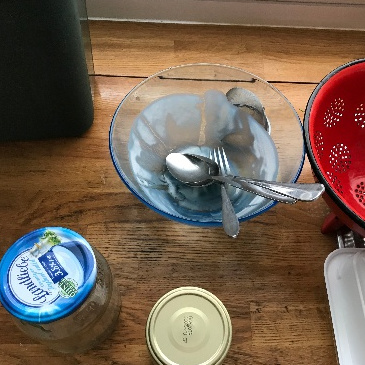
\includegraphics[width=0.31\textwidth]{demo_query.jpg}\hfill
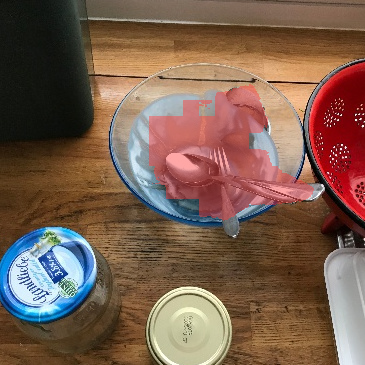
\includegraphics[width=0.31\textwidth]{demo_text.png}\hfill
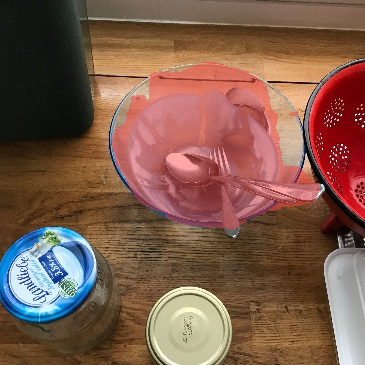
\includegraphics[width=0.31\textwidth]{demo_visual.png}
\caption{Kiểm tra inference ban đầu: ảnh query từ repo tác giả~\cite{clipsegcode}, text ``a spoon'' và visual crop cùng ảnh. Ví dụ này chưa có GT và không dùng làm kết quả E2.}
\label{fig:smoke}
\end{figure}
[Thay hoặc bổ sung các hình có GT để phân tích vật nhỏ, nhiều vật, thuộc tính và quan hệ.]

\chapter{Kết luận và hướng phát triển}
\section{Kết quả đạt được}
[Tóm tắt kết quả đã đo của E1--E3 và phần triển khai. Mỗi kết luận phải gắn với bảng hoặc hình trong báo cáo.]

\section{Hạn chế}
[Nêu giới hạn tập con, checkpoint, ngưỡng, ảnh support và tính công bằng của các so sánh.]

\section{Hướng phát triển}
[Đề xuất một hoặc hai hướng có căn cứ từ lỗi đã quan sát, chẳng hạn đánh giá lớn hơn hoặc kết hợp bước tinh chỉnh mask.]

\chapter*{Tài liệu tham khảo}
\addcontentsline{toc}{chapter}{Tài liệu tham khảo}
\printbibliography[heading=none]
\end{document}
